\documentclass{article}

\usepackage{amsmath}
\usepackage{amssymb}
\usepackage{amsfonts}
\usepackage{mathtools}

\usepackage[thmmarks, amsmath]{ntheorem}

\usepackage{graphicx}
\usepackage{float}
\usepackage{tikz}
\usetikzlibrary{positioning}

\usepackage{fullpage}

\usepackage{cancel}
\usepackage{interval}

\usepackage{enumitem}

\setlist[enumerate,1]{label=\alph*)}

\title{On Small Models of Theories}
\author{Duarte Maia}
%\date{}

\theorembodyfont{\upshape}
\theoremseparator{.}
\newtheorem{theorem}{Theorem}[subsection]
\newtheorem{prop}[theorem]{Proposition}
\renewtheorem*{prop*}{Proposition}
\newtheorem{lemma}[theorem]{Lemma}
\newtheorem{remark}[theorem]{Remark}
\newtheorem{example}[theorem]{Example}

\theoremsymbol{\ensuremath{\square}}
\newtheorem{prelimdef}[theorem]{Preliminary Definition}
\newtheorem{definition}[theorem]{Definition}

\theoremstyle{nonumberplain}
\theoremsymbol{}
\newtheorem{convention}{Convention}

\theoremheaderfont{\itshape}
\theorembodyfont{\upshape}
\theoremseparator{:}
\theoremsymbol{\ensuremath{\blacksquare}}
\newtheorem{proof}{Proof}

\theoremsymbol{\ensuremath{\square}}
\newtheorem{sketch}{Proof Sketch}

\newcommand{\N}{\mathbb{N}}
\newcommand{\Z}{\mathbb{Z}}
\newcommand{\Q}{\mathbb{Q}}
\newcommand{\R}{\mathbb{R}}
\newcommand{\C}{\mathbb{C}}

\newcommand{\CF}{\mathrm{CF}}
\newcommand{\Seq}{\mathrm{Seq}}

\newcommand{\upcl}[1]{{#1}\hspace{-0.25em}\uparrow}
\newcommand{\dncl}[1]{{#1}\hspace{-0.25em}\downarrow}

\DeclarePairedDelimiter{\braket}{\langle}{\rangle}
\DeclarePairedDelimiter{\abs}{\lvert}{\rvert}



\begin{document}
\maketitle

\tableofcontents

\section{Introduction}

\begin{convention}
Unless otherwise specified, we will be working with models over a countable language.
\end{convention}

As of the time of writing this document, the author is aware of two prior existing (equivalent) characterizations of what it means for a model $M$ (of a complete theory $T$) to be `as small as possible'. One of these is for the model to be \emph{atomic}, that is, any finite tuple of elements of $M$ satisfies a $T$-complete formula. Another is for the model to be prime, that is, for it to embed elementarily into any other model of $T$.

In the process of studying these notions, I came up with my own notion of smallness of a model, which I was easily able to show agrees with the the notions above in the case where $T$ is an atomic theory. I harbored some hope that my notion of smallness might be a (fruitful?) generalization of them to the nonatomic case. This turned out not to be so: the notion of smallness I came up with wound up being precisely equivalent to being atomic.

In this document, I will attempt to motivate my definition of a model $M$ being `small'\footnote{Since my notion adds nothing new, I opted not to give it a better name.} and show the path I took in showing that this notion is equivalent to atomicness.

As a last remark before beginning, this was all done in the context of countable languages, which is the context where all I know about atomic models holds. It might be the case that my notion is fruitful in contexts with larger languages (though I find it more likely that it is still equivalent to atomicness), but I would prefer to learn more about larger languages before venturing in such directions.

\section{The Main Definition}

\subsection{Introduction}

As motivation for our main definition, let us think for a little about the question: What elements must a model $M$ of a theory $T$ have for sure?

To first approximation, the only things that $T$ can guarantee exist are witnesses to existential formulas $\exists_x \varphi(x)$ which hold in $T$. As such, one might identify a property of a small model to be: every element is there to witness some existential statement. Unfortunately this proves far too weak, as any element certainly witnesses \emph{some} existential statement, e.g. $x = x$.

To remedy this issue, we may instead shift gears to: to each existential statement, we associate to it a witness in $M$. This then becomes the witness's \textit{raison d'etre}, and so we demand that every element of $M$ has such a reason to exist. Formally, our first definition of small model becomes:
\begin{prelimdef}\label{pd:1}
If $M$ is a model of the complete theory $T$, we say that $M$ is small if there is a \emph{surjective} map $W$ from the formulas in one free variable which are consistent with $T$ (i.e. the formulas $\varphi(x)$ such that $T \vdash \exists_x \varphi(x)$) to the model, such that $m = W(\varphi)$ always satisfies $M \Vdash \varphi[m]$.
\end{prelimdef}

The collection of formulas defined above will be useful in the future, so we give it (and its higher arity cousins) a name.
\begin{definition}
In the context of a given complete theory $T$, denote by $\CF_n$ the set of formulas in $n$ free variables which are consistent with $T$, that is,
\begin{equation}
\CF_n := \{\, \varphi(x_1, \dots, x_n) \mid T \vdash \exists_{\vec x} \varphi(\vec x) \,\}.
\end{equation}
\end{definition}

There are a few problems with Preliminary Definition \ref{pd:1}:
\begin{itemize}
\item It still allows for large amounts of redundancy, given that we have infinitely many distinct true sentences, e.g. $x=x$, $x=x \land x=x$, etc. Thus, any countable model admits such a surjective map $W$.

This can be remedied by making the reasonable demand that equivalent formulas have the same witness, but this might not be sufficient to avoid subtler manifestations of the same issue, which we will henceforth refer to in general as \emph{redundancy}. Avoiding redundancy is the main content of our definition, and we will go into greater depth shortly.

\item Under the light (but essential) assumption that equivalent formulas have the same witness, it might be impossible for $W$ to be surjective. For instance, consider the theory of a dense linear order with no endpoints, in which up to equivalence there is exactly one formula in one free variable.

To remedy this issue, we weaken the requirement for surjectivity. To motivate the weakening, we return for the theory of a dense linear order with no endpoints. Then, we may attempt to justify that $\Q$ is a model with as few elements as possible via the following process.

First, there must be a witness to $x = x$, so we pick some witness $q_0 = W(x=x)$. Then, there must be a witness (or rather a pair of witnesses) to $x<y$, so we pick two elements $q_1 < q_2$ (one of which may or may not equal $q_0$). Then, we must also have a witness to $x<y \land y<z$, and so on. If we proceed in an appropriate way, we may ensure that every element of $\Q$ is there to witness one of these formulas, which is a light plausibility argument for smallness of $\Q$ as a model.

This motivates the idea that our elements may need to exist not just to witness formulas of the form $\exists_x \varphi(x)$, but also $\exists_{x_1, \dots, x_n} \varphi(x_1, \dots, x_n)$. In turn, this suggests defining $W$ to act on existential formulas of \emph{any} arity, and weakening our notion of surjectivity to what we will call \emph{surjectivity up to padding}.
\end{itemize}

\begin{definition}[Witnessization, Surjectivity up to Padding]
Let $M$ be a model of $T$, and let $W$ be a collection of functions $W_n \colon \CF_n \to M^n$, for $n \in \N$. We call such a collection of functions a \emph{witnessization of $M$}.

We say that such a $W$ is \emph{(strongly) surjective up to padding} (shortened to `suptop') if, for every $n$-uple $\vec m = (m_1, \dots, m_n)$ of elements of $M$, there is some $N$-uple $\vec\mu = (\mu_1, \dots, \mu_N)$ in the image of $W_N$, of which $\vec m$ is a subtuple, or equivalently, such that $\vec\mu$ is a padding of $\vec m$. For our purposes, let us say that the ordering must be preserved in the subtuple relation, though this will not be relevant.

We say that $W$ is \emph{weakly surjective up to padding} (shortened to `weak suptop') if the above condition holds for $n = 1$.
\end{definition}

\subsection{Avoiding Redundancy}

Let us now investigate the following question: How to characterize the redundancy of a witnessization $W$?

We have already identified a measure in which $W$ might be redundant, namely: If $T \vdash \forall_{\vec x}  (\varphi(\vec x) \leftrightarrow \psi(\vec x))$, we expect that $W(\varphi) = W(\psi)$.

Another attempt to avoid redundancy is as follows: $W(\varphi \lor \psi)$ should agree with either $W(\varphi)$ or $W(\psi)$. This is because, if we already have a witness to these two formulas, we do not need to look elsewhere to find a witness to $\varphi \lor \psi$; either of these two witnesses will do.

While this property is already pretty strong, it is not our final demand, because it is too finitary in nature. Indeed, it might happen that a formula $\varphi$ is, morally speaking, equivalent to a disjunction of infinitely many other formulas $\varphi_1$, $\varphi_2$ etc., in which case we still want $W(\varphi)$ to agree with $W(\varphi_k)$ for some $k$. This leads us to our first serious demand for nonredundancy, for which we first need to introduce some notation.
\begin{definition}
Let $S$ be a subset of $\CF_n$. Then, we say $\varphi \in \CF_n$ is the join of $S$, denoted by abuse of notation $\varphi \equiv \bigvee S$, if for all $\alpha \in \CF_n$ such that $T \vdash \sigma \rightarrow \alpha$ for every $\sigma \in S$, we have $T \vdash \varphi \rightarrow \alpha$.
\end{definition}

\begin{remark}
The above definition is simply the standard definition of the join\slash supremum\slash least upper bound of a subset of a poset, applied to the poset of consistent formulas modulo equivalence.

In particular, any two joins of $S$ are equivalent.
\end{remark}

\begin{remark}
We make no assumptions on the existence of joins of sets, and thus the symbol $\bigvee S$ might not make sense. Joins of finite nonempty(!) sets always exist, though: simply consider the disjunction of all elements of the set.
\end{remark}

\begin{remark}\label{rmk:shaky}
This notion of join of a collection of formulas has weird model-theoretic repercussions, or rather lack thereof. Indeed, if $\varphi \equiv \bigvee S$ in a nonfinite way (i.e. for no finite subset $\{\sigma_1, \dots, \sigma_n\}\subseteq S$ do we have $\varphi \equiv \bigvee \sigma_k$), then there always exists a model of $T$ containing some element satisfying all $\sigma \in S$, but not $\varphi$. Thus, the interpretation of the join as an infinitary disjunction is shaky.
\end{remark}

We may now make our first main definition:
\begin{definition}\label{def:nr1j}
Let $W$ be a witnessization of a model $M$ of a theory $T$. We say that $W$ satisfies the \emph{join variant of the first nonredundancy condition}, abbreviated to `$W$ satisfies \eqref{eq:nr1j}', if
\begin{equation}
\tag{NR1-J}\label{eq:nr1j}
\begin{tabular}{ll}
For all $S \subseteq \CF_n$ and $\varphi \in \CF_n$,\\
if $\varphi \equiv \bigvee S$ then there is some $\sigma \in S$ such that $W(\varphi) = W(\sigma)$.
\end{tabular}
\end{equation}
\end{definition}

I would like to criticize the above the definition for a moment. Besides the sentence at the end of remark \ref{rmk:shaky}, there is something that irks me about definition \ref{def:nr1j}: it appears too strong. Again, by the content of remark \ref{rmk:shaky}, joins do not correspond necessarily to infinitary disjunctions, and while it seems perhaps plausible that they would agree in a `small enough' model, this is not a foregone conclusion. Thus, I temporarily discard condition \eqref{eq:nr1j} in favor of condition \eqref{eq:nr1} below, which to me appears a milder requirement.

The entirety of the above paragraph will be invalidated when I show that \eqref{eq:nr1j} and \eqref{eq:nr1} are equivalent, in section \ref{sec:nr1jeqvnr1}

Before we move on, a quick sanity check

\begin{lemma}
If $W$ is a witnessization satisfying \eqref{eq:nr1j}, it maps equivalent formulas to the same witness. Moreover, $W(\varphi \lor \psi) \in \{W(\varphi), W(\psi)\}$.
\end{lemma}

\begin{proof}
For the first part, apply \eqref{eq:nr1j} to $S = \{\psi\}$. For the second part, apply \eqref{eq:nr1j} to $S = \{\varphi, \psi\}$.
\end{proof}

\subsection{Avoiding Redundancy (Reprise)}

Let us now investigate an alternative way to characterize nonredundancy.

The definition we introduce in this section is in fact my original definition of nonredundancy, and while I believe that it is a more reasonable definition than \eqref{eq:nr1j}, the fact that it will require an entire section dedicated to its motivation is a sign that it is not as clean a definition as it should be. On the other hand, the fact that it is equivalent to \eqref{eq:nr1j} (see section \ref{sec:nr1jeqvnr1}), and that the existence of a suptop witnessization of $M$ satisfying either of these two is equivalent to $M$ being atomic (section \ref{sec:mainresult}), indicates that there is a reasonably canonical and unequivocal notion of small model, which all three of these definitions manage to encapsulate. As such, while in isolation I am not able to map either of the three definitions cleanly to my intuitive notion of small model, the fact that the same definition has come up thrice from different directions is enough to persuade me that they all encapsulate the correct notion of smallness.

In spite of the previous paragraph, I feel that all three of the definitions under inspection are a little bit stronger than my intuitive notion of `smallest possible model', and I still harbor some hope for a slightly weaker definition of small model. See section \ref{sec:evensmaller} for (slightly) more detail.

\smallskip

The main step in our definition is defining what it means for a set $S$ to `cover $\varphi$ from below' in some reasonable sense, that we may believe that if a witness to $\varphi$ exists, one may be found to be also a witness of an element of $S$. We begin with a concrete example for what such an $S$ might be.

\begin{example}\label{ex:indepunary}
Consider the theory with countably many independent unary predicates. Then, it can be shown that the only formulas (in one variable) are, up to equivalence, a disjunction of conjunctions of either $p(x)$ or $\neg p(x)$. Ignoring the disjunctions for now, we may look at the poset which has $\top$ at the very top, then a layer below that which has all formulas $p(x)$ and $\neg p(x)$, and a layer below that with all binary combination $p(x) \land q(x)$, etc. Then, whatever the witness of $\top$ is, we expect it to satisfy some predicate $p(x)$ or its negation. Thus, a witnessization of minimal redundancy would be expected to reuse $W(\top)$ as the witness of some predicate. Likewise for a conjunction of two predicates, and so on.
\begin{figure}[H]
\centering
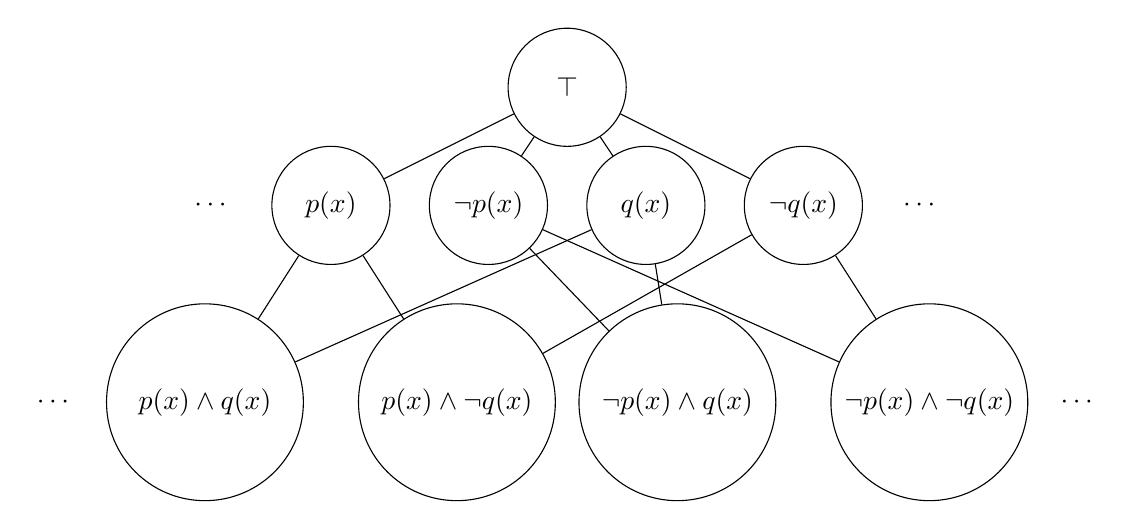
\begin{tikzpicture}[node/.style={draw,circle, minimum size=1.5cm}, node2/.style={node, minimum size=2.5cm}]
\node[node] (T) at (0,0) {$\top$};
\node[node] (P) at (-3,-1.5) {$p(x)$};
\node[node] (NP) at (-1,-1.5) {$\neg p(x)$};
\node[node] (Q) at (1,-1.5) {$q(x)$};
\node[node] (NQ) at (3,-1.5) {$\neg q(x)$};

\node[node2] (PQ) at (-4.6, -4) {$p(x) \land q(x)$};
\node[node2] (PNQ) at (-1.4, -4) {$p(x) \land \neg q(x)$};
\node[node2] (NPQ) at (1.4, -4) {$\neg p(x) \land q(x)$};
\node[node2] (NPNQ) at (4.6, -4) {$\neg p(x) \land \neg q(x)$};

\node at (-4.5, -1.5) {$\cdots$};
\node at (4.5, -1.5) {$\cdots$};
\node at (-6.5, -4) {$\cdots$};
\node at (6.5, -4) {$\cdots$};

\draw (T)--(P);
\draw (T)--(NP);
\draw (T)--(Q);
\draw (T)--(NQ);

\draw (P)--(PQ);
\draw (P)--(PNQ);
\draw (NP)--(NPQ);
\draw (NP)--(NPNQ);
\draw (Q)--(PQ);
\draw (NQ)--(PNQ);
\draw (Q)--(NPQ);
\draw (NQ)--(NPNQ);
\end{tikzpicture}
\caption{Part of $\CF_1$ for the theory of independent unary predicates.}
\end{figure}

Note that this is, in principle, far weaker than the requirement that $W(\varphi \lor \psi) \in \{W(\varphi), W(\psi)\}$: this would actually imply that $W(\top)$ appears in each layer infinitely many times, once for each pair $p(x)$, $\neg p(x)$.
\end{example}

Now it remains to try to abstract in what sense does each of these layers `cover the above from below'. For clarity, we now work in a more abstract setting: let $P$ be a poset (represeting $\CF_n$ mod equivalence), let $a \in P$, and let $S \subseteq P$. We will attempt to define the notion `$S$ covers $a$ from below'.

\begin{prelimdef}\label{pdef:below1}
Intuitively, one may think of $S$ covering $a$ from below if `any unbroken thread starting from $a$ and going infinitely downwards inevitably meets $S$'. It remains to define this notion of `unbroken thread'.

We define a `rope descending from $a$' as a maximal linearly ordered subset containing $a$. Equivalently\footnote{This requires a quick Zorn's lemma argument.}, we say that $C \subseteq P$ is a rope descending from $a$ if it satisfies
\begin{enumerate}
\item\label{item:rope1} $a \in C$,
\item\label{item:rope2} (Unbrokenness) If $A, B \subseteq C$ and there is some $p \in P$ satisfying $A < p < B$ (that is, $\forall_{a \in A} \forall_{b \in B} a < p < b$), then there is some $p \in C$ satisfying $A < p < B$,
\item\label{item:rope3} (Infinitely descending) There is no $p \in P$ with $p < C$. 
\end{enumerate}

Then, we say that $S$ covers $a$ from below if any rope descending from $a$ intersects $S$.
\end{prelimdef}

This definition may be interesting in its own right, but it is too weak to let us capture the notion of small model, and the problem is with the notion of infinitely descending. To understand the problem, we provide two examples.

\begin{example}\label{ex:ex1}
Consider the following ordering on $\R^2$, which will be useful for diagrammatic purposes. Given a point $p \in \R^2$, draw two diagonal lines passing through $p$, with slopes $\pm 1$. This splits the plane into four infinite cones. We say that the elements in the cone above $p$ are those which are greater than or equal to $p$, and in the cone below $p$ we have the elements less than or equal to $p$.
\begin{figure}[H]
\centering
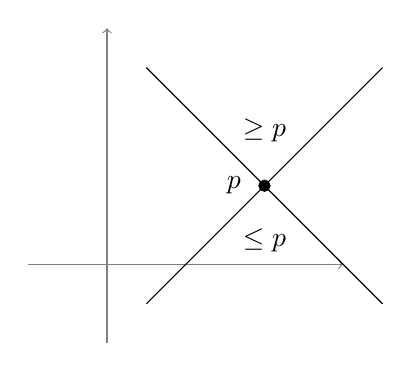
\begin{tikzpicture}
\draw[->,gray] (-1,0)--(3,0);
\draw[->,gray] (0,-1)--(0,3);

\node[draw,circle,fill=black,inner sep=0.05cm] (P) at (2,1) {}; 
\node[left=0.1cm of P] {$p$};

\draw (P)+(-1.5,-1.5) --+ (1.5,1.5);
\draw (P)+(1.5,-1.5) --+ (-1.5,1.5);

\draw (P)+(0,0.7) node {$\geq p$};
\draw (P)+(0,-0.7) node {$\leq p$};
\end{tikzpicture}
\caption{Schematic representation of the ordering in $\R^2$.}
\end{figure}

Formally, we say $p$ and $q$ are comparable if $\abs{p_x - q_x} \leq \abs{p_y - q_y}$, in which case we compare them by their $y$ coordinate.

Now, consider the poset $P \subseteq \R^2$, given by $P = \ointerval01 \times \interval01$ with the subset ordering. Then, the base of the square $S = \ointerval01 \times 0$ does not cover $p = (\frac12, 1)$ from below; figure \ref{fig:ex1} shows an example of a rope $C$ which proves that this is the case. We will see in example \ref{ex:ex2} why this is undesirable.
\begin{figure}[H]
\centering
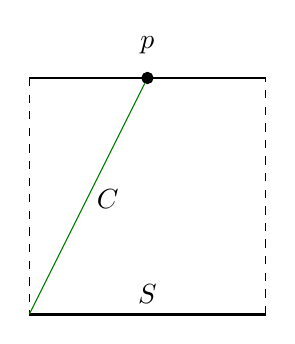
\begin{tikzpicture}[scale=3]
\draw[very thick] (0,0) -- (1,0) node[midway, above] {$S$};
\draw[dashed] (1,0) -- (1,1);
\draw (1,1) -- (0,1);
\draw[dashed] (0,1) -- (0,0);


\node[draw,circle,fill=black,inner sep=0.05cm] (P) at (0.5,1) {}; 
\node[above=0.1cm of P] {$p$};

\draw[green!50!black] (P) -- (0,0) node[midway, text=black, right] {$C$};
\end{tikzpicture}
\caption{Example which shows an unintended repercussion of Preliminary Definition \ref{pdef:below1}.}\label{fig:ex1}
\end{figure}
\end{example}

Now we show a more concerning example.

Recall that the notion of `$S$ covers $a$ from below' which we are trying to define intends to yield a criterion to allow us to say that, if witnesses to formulas have been chosen in a minimally redundant way, the witness to $a$ will have been chosen as the witness of some element of $S$. The following example shows that Preliminary Definition \ref{pdef:below1} fails to serve as such a criterion.

\begin{example}\label{ex:ex2}
Consider the theory $T$ of the natural numbers as an ordered set, and let $M$ be a nonstandard model. Let $m \in M$ be a nonstandard element. Let $P$ be the poset given by $\CF_1$ modulo equivalence, $a = \top$, and $S$ the collection of formulas (morally equivalent to) $x = 0$, $x = 1$, etc.

It is clear that any formula in $P$ has a witness which is a witness of some element in $S$, so it is desirable that our definition makes $S$ cover $a$ from below. We will now see that this is not the case.

Let $C_0$ be the set of formulas satisfied by $m$ (or indeed, by any nonstandard element). This set is not linearly ordered, but it otherwise satisfies properties \ref{item:rope1}, \ref{item:rope2}, and \ref{item:rope3} in the definition of rope\footnote{This statement is mostly trivial, but showing \ref{item:rope3} requires a bit of thought. A sketch goes as follows: Given a formula $p \in \CF_1$, it is satisfied by some natural number $n$. Then, $p$ does not imply the formula `$x$ has at least $n+1$ distinct elements below it', which is in $C$.}. An argument by Zorn's lemma will show that we may then find a linearly ordered subset $C \subseteq C_0$ which forms a rope descending from $a$. Finally, it is obvious that $C_0$, and hence $C$, does not intersect $S$, which proves that $S$ does not cover $a$ from below as per Preliminary Definition \ref{pdef:below1}.
\begin{figure}[H]
\centering
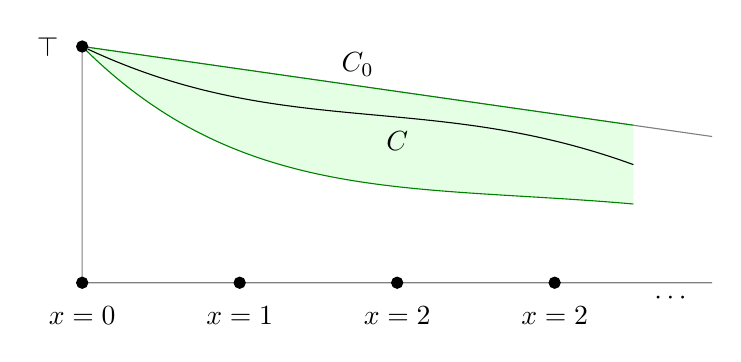
\begin{tikzpicture}

\draw[gray] (8,0) -- (0,0) -- (0,3) -- (8,1.857);

\node[draw,circle,fill=black,inner sep=0.05cm] (X0) at (0,0) {}; 
\node[below=0.1cm of X0] {$x = 0$};
\node[draw,circle,fill=black,inner sep=0.05cm] (X1) at (2,0) {}; 
\node[below=0.1cm of X1] {$x = 1$};
\node[draw,circle,fill=black,inner sep=0.05cm] (X2) at (4,0) {}; 
\node[below=0.1cm of X2] {$x = 2$};
\node[draw,circle,fill=black,inner sep=0.05cm] (X3) at (6,0) {}; 
\node[below=0.1cm of X3] {$x = 2$};

\node at (7.5,-0.2) {$\cdots$};

\draw[green!50!black, fill=green!10] (7,2) -- (0,3) node[midway, above, text=black] {$C_0$} to[out=-45, in=175] (7,1);

\node[draw,circle,fill=black,inner sep=0.05cm] (T) at (0,3) {}; 
\node[left=0.1cm of T] {$\top$};

\draw (T) to[out=-25, in=160] (7,1.5);
\node at (4,1.8) {$C$};
\end{tikzpicture}
\caption{Schematic representation of example \ref{ex:ex2}.}\label{fig:ex2}
\end{figure}
\end{example}

By looking at examples \ref{ex:ex1} and \ref{ex:ex2}, we understand that something is lacking in our definition of `covers from below'. The problem is that a rope descending from $a$ might just barely avoid ever touching $S$, by going `infinitely to the side'. Thus, a definition of belowness based on ropes is likely doomed to fail.

Let us try another angle. An important property of the sets $S$ in the above examples is that they form a `floor' to the poset $P$, in the sense that for any element $p \in P$ there is some $s \in S$ such that $s \leq p$. Given such a set $S$, we will thus want the witness of $p$ to be chosen as the witness to some element of $S$.

\begin{definition}
Given an element $s$ of the poset $P$, we define the upper closure $\upcl s$ as the set
\begin{equation}
\upcl s := \{\,p \in P \mid p \geq s\,\}.
\end{equation}

The lower closure $\dncl s$ is defined analogously.
\end{definition}

\begin{prelimdef}
We say that $S$ covers $a$ from below if $\dncl a \subseteq \bigcup_{s \in S} \upcl s$.
\end{prelimdef}

This is unfortunately still insufficient, as example \ref{ex:indepunary} shows. More generally, it only suffices to embody the notion of a `floor' of a poset, when what we want is to embody the notion of a set that separates the poset into an `above' and a `below'. However, a path forward now becomes clear: given a set $S$, its `above' is $\bigcup_{s \in S} \upcl s$, and its `below' as $\bigcup_{s \in S} \dncl s$, and thus:

\begin{definition}
Let $P$ be a preorder, $a \in P$, and $S$ a subset of $\dncl a$. We say that $S$ covers $a$ from below if
\begin{equation}
\dncl a \subseteq \left( \bigcup_{s \in S} \upcl s \right) \cup \left( \bigcup_{s \in S} \dncl s \right).
\end{equation}

In other words, we say $S$ covers $a$ from below if any element of $\dncl a$ is comparable to some element of $S$.
\end{definition}

\begin{remark}
Note that we have made the above definition for a preorder instead of a poset. This will allow us to work in the preorders $\CF_n$ without having to identify formulas modulo equivalence.
\end{remark}

\begin{definition}
Let $W$ be a witnessization of a model $M$ of a theory $T$. We say that $W$ satisfies the \emph{first nonredundancy condition}, abbreviated to `$W$ satisfies \eqref{eq:nr1}', if
\begin{equation}
\tag{NR1}\label{eq:nr1}
\begin{tabular}{ll}
For all $\varphi \in \CF_n$ and $S \subseteq \dncl\varphi$,\\
if $S$ covers $\varphi$ from below, then there is some $\sigma \in S$ such that $W(\varphi) = W(\sigma)$.
\end{tabular}
\end{equation}
\end{definition}

\subsection{A Study of \eqref{eq:nr1}}

\begin{definition}
Let $M$ be a model of a theory $T$. We say that $M$ is \emph{small} if there exists a suptop witnessization $W$ which satisfies \eqref{eq:nr1}.

By abuse of language, we will say `let $M$ be a small model and let $W$ be its witnessization' to mean that $W$ is a suptop nonredundant witnessization of $M$.
\end{definition}

We begin by showing that smallness coincides with atomicness in the case that the theory $T$ is itself atomic.

\begin{prop}\label{thm:mainresult0}
Let $M$ be a model of the atomic theory $T$. Then $M$ is small iff it is countably atomic.
\end{prop}

\begin{proof}
($\rightarrow$) The proof that $M$ is countable uses the fact that the cardinality of $M$ is bounded from above by $\# \bigcup \CF_n \leq \aleph_0^2 = \aleph_0$.

Now, we show that $M$ is atomic. Let $\vec m$ be a tuple of elements of $M$. By surjectivity up to padding, one may pad $\vec m$ into a vector $\vec \mu$ which satisfies $\vec \mu = W(\varphi)$ for some $\varphi(x_1, \dots, x_N)$. Now, let $S$ be the collection of complete formulas in $N$ variables (in the theory $T$) which imply $\varphi$. We claim that the fact that $T$ is atomic implies that $S$ covers $\varphi$ from below.

Indeed, let $\alpha \in \CF_n$ such that $T \vdash \alpha \rightarrow \varphi$. Since $T$ is atomic, there is some complete formula $\sigma$ such that $T \vdash \sigma \rightarrow \alpha$. We just need to show that $\sigma \in S$, i.e. that $T \vdash \sigma \rightarrow \varphi$. But if not, then $T \vdash \sigma \rightarrow \neg \varphi$, and hence $T \vdash \sigma \rightarrow \neg \alpha$, a contradiction.

Now, applying \eqref{eq:nr1}, we conclude that $\vec\mu = W(\sigma)$ for some complete formula in $N$ variables, and so in particular $T \vdash \sigma(\vec\mu)$. Quantifying existentially over all the variables that were used to pad $\vec m$ into $\vec \mu$, we obtain a complete formula satisfied by $\vec m$.

\medskip

($\leftarrow$) Suppose that $M$ is countably atomic. Then, order it by a countable cardinal, say $M = \{m_0, m_1, \dots\}$, and set $W(\varphi(x_1, \dots, x_n))$ to be the lexicographically smallest $n$-uple of elements of $M$ which satisfies $\varphi$. We claim that this is a suptop witnessization of $M$ which satisfies \eqref{eq:nr1}.
\begin{itemize}
\item (Suptop) For simplicity, we show simply that any pair of elements $(m_a, m_b)$ is attained up	to padding. The argument generalizes trivially to larger tuples; the notation does not.

Consider the formula
\begin{equation}
\varphi(x_1, \dots, x_{a+b+2}) \colon (\text{$x_1, \dots, x_{a+1}$ are distinct}) \land (\text{$x_{a+2}, \dots, x_{a+b+2}$ are distinct}).
\end{equation}

Then, $W(\varphi)$ is given by the tuple
\begin{equation}
W(\varphi) = (m_0, \dots, m_a, m_0, \dots, m_b),
\end{equation}
which is a padding of $(m_a,m_b)$.

\item (\ref{eq:nr1}) Let $\varphi \in \CF_n$, and let $S \subseteq \dncl\varphi$ cover $\varphi$ from below. We find some $\sigma \in S$ such that $W(\sigma) = W(\varphi)$.

Let $\theta$ be a complete formula such that $T \vdash \theta \rightarrow \varphi$. By definition of covering from below, we find $\sigma \in S$ which is comparable to $\theta$. It is easy to argue that indeed $T \vdash \theta \rightarrow \sigma$, and so in particular $M \vDash \sigma[W(\varphi)]$. Hence, $W(\sigma) \leq W(\varphi)$ in the lexicographical order. But on the other hand, since $T \vdash \sigma \rightarrow \varphi$ we also have $W(\varphi) \leq W(\sigma)$, and so indeed $W(\sigma) = W(\varphi)$.
\end{itemize}
\end{proof}

We now show some smaller results.

\begin{prop}
If $W$ is a witnessization satisfying \eqref{eq:nr1}, it maps equivalent formulas to the same witness. Moreover, $W(\varphi \lor \psi) \in \{W(\varphi), W(\psi)\}$.
\end{prop}

\begin{proof}
For the first part, suppose that $T \vdash \varphi \leftrightarrow \psi$. Then, simply note that $\varphi$ is covered from below by $S = \{\psi\}$.

The second part is a little more complicated. To begin, set $\vec m = W(\varphi \lor \psi)$. Then, either $M \vDash \varphi[\vec m]$ or $M \vDash \psi[\vec m]$. Supposing without loss of generality the first case, we show that $W(\varphi) = \vec m$.

Define $S$ as the set
\begin{equation}
S = \{\varphi\} \cup \{\, \neg\varphi \land \alpha \mid \alpha \in \dncl\psi, (\neg\varphi \land \alpha) \in \CF_n\,\}.
\end{equation}

Then, by \eqref{eq:nr1}, if we show that $S$ covers $\varphi \lor \psi$ from below, we immediately have that $W(\varphi \lor \psi) = W(\sigma)$ for some $\sigma \in S$, and it is evident that this $\sigma$ may only be $\varphi$.

Thus, suppose that $\alpha \in \dncl{(\varphi \lor \psi)}$. We show that $\alpha$ is comparable to some element of $S$. If $T \vdash \alpha \rightarrow \varphi$ we are done. Otherwise, $T \vdash \exists_{\vec x}(\alpha \land \neg\varphi)$, hence $(\neg\varphi \land\alpha) \in \CF_n$. Hence, the formula $\neg\varphi \land\alpha$, which obviously implies $\alpha$, is in $S$. This concludes the proof.
\end{proof}

\subsection{Smallness and Atomicness are Equivalent}\label{sec:mainresult}

We saw in Proposition \ref{thm:mainresult0} that, if the theory $T$ is atomic, a model is small iff it is countably atomic. This still leaves open the possibility that, if $T$ is not atomic, a model is small without being atomic. We now crush any such hopes. (Rephrase)

\subsection{\eqref{eq:nr1j} and \eqref{eq:nr1} are Equivalent}\label{sec:nr1jeqvnr1}

\subsection{Second Nonredundancy Conditions}

\subsection{On the Ease of Too Strong Smallness Definitions}

\section{Possible Further Avenues}

\subsection{Large Languages}

\subsection{There May be a Weaker Notion of Small}\label{sec:evensmaller}


%\bibliographystyle{plain}
%\bibliography{bibliography}

\end{document}